%************************************************
\chapter{Introduction}\label{ch:introduction}
%************************************************

In recent years, we have witnessed an unprecedented level of presence of technology in our lives. Mobile phones are smarter every day, with computational power that overtakes desktop computers just a couple of years old. At the same time, these devices gain in ubiquity as they extend their functionality to wearable technology, e.g. wearable cameras, wireless earphones or smart watches. The cameras installed in these devices have seen a similar increase in presence, resolution and quality of the lenses and sensors.

The combination of better cameras with improved processing and network connectivity opens the possibilities for computer vision to contribute to diverse applications, some of them having a special role in the inclusivity of people with disabilities and a positive impact in quality of life.

The diagram shown in Figure~\ref{fig:cv_dev_pipeline} illustrates a flow chart that depicts the process behind the development of an application that might depend on computer vision algorithms. In brief, this entails the development of a prototype that is later refined with the use of data. 

Data is the cornerstone for parameter optimisation and at the same time for applying the learning methods that are increasingly being made in many approaches that rely on artificial intelligence. Within computer vision, data, and in particular annotated data, has driven research very strongly. The availability of annotated datasets has achieved prominence, with the organisation of systematic and objective challenges around object recognition and detection; examples include PASCAL VOC \cite{everingham2010pascal} and ImageNet \citep{Deng2009}). Through these data collections and open competitions, benchmaarks for performance have been established that are now being extended to other fields within computer vision such as navigation (NAVVIS \cite{Huitl2012} and SLAMbench \cite{nardi2014introducing}.

In recent years, \textit{big data}, or the use of massive amounts of structured and unstructured data has made learning and prediction algorithms an important piece of the artificial intelligence puzzle. However, relying almost entirely in the use of data to solve the problem has sometimes caused the loss of perspective and very poor improvements on performance or none at all \cite{zhu2012we}. It is therefore to keep developing core algorithms and richer models that help solve artificial intelligence problems by gaining a better understanding of their constraints and representational structure. Often the solution is closer than what we think, and biology can provide us with efficient models that solve the problem in an effective way. In particular, in computer vision, models of the visual system have been shown to be effective in key tasks such as object recognition and visual localisation \cite{lowe2004distinctive,milford2004ratslam}. 


\begin{figure}
\centering
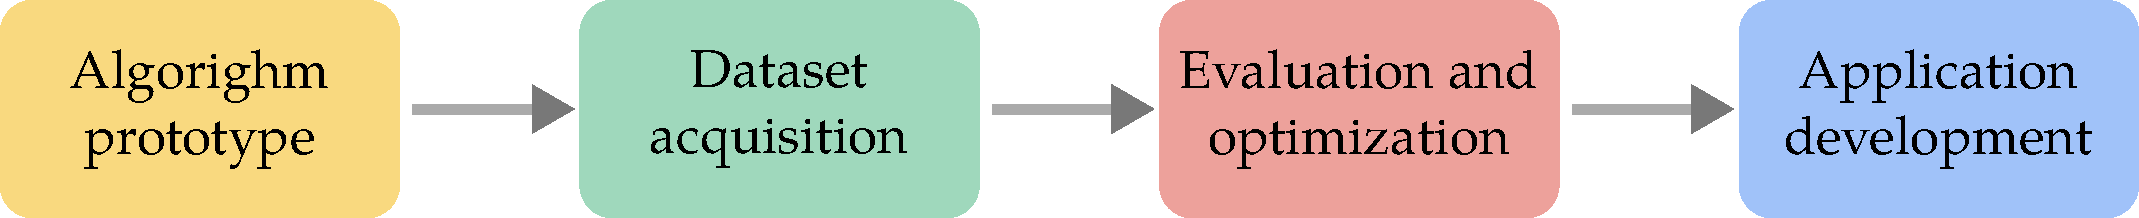
\includegraphics[width=\linewidth]{gfx/Chapter01/cv_dev_pipeline.pdf}
\caption{Stages in the development of a computer vision application. The development of an application in computer vision and similar artificial intelligence disciplines requires a different form of testing compared to the ones seen in standard software engineering toolchains. The use of databases and evaluation and optimisation stages prior to the development of the application complements the typical deterministic behaviour test suites.}
\label{fig:cv_dev_pipeline}
\end{figure}


This thesis represents 

\section{Organisation of the thesis}

The remainder of this dissertation is organised as follows: Chapter 2 presents our motivation on the acquisition of datasets and early work on appearance-based methods for visual localisation. Chapter 3 describes the SHORT dataset, a dataset for hand-held object recognition with an emphasis on the assistive context. Chapter 4 introduces our evaluation benchmark of descriptors for visual localisation. Chapter 5 presents our biologically inspired framework for visual localisation. In addition, we show experimental results of place-cells localisation  and a comparison with state-of-the-art SLAM. Chapter 6 describes our assistive vision-based localisation App that uses a wearable camera and a haptic feedback tablet to provide basic positional information. Finally in Chapter 7 we provide concluding remarks while summarising the main contributions of this dissertation and future work.


